\documentclass[12pt,a4paper,onecolumn,oneside]{extreport}

%/usr/texbin/latex -interaction=nonstopmode %.tex|/usr/texbin/bibtex %.aux|/usr/texbin/latex -interaction=nonstopmode %.tex|/usr/texbin/latex -interaction=nonstopmode %.tex

%\usepackage{times}
\usepackage{amsmath}
\usepackage{amssymb}
\usepackage[utf8x]{inputenc}
\usepackage[T1]{fontenc}
\usepackage[polish]{babel}
\usepackage{graphicx}
\usepackage{url}
\usepackage[ruled, vlined, polish]{algorithm2e-pl}
\usepackage{setspace}
\usepackage{tocbibind}
\usepackage{fancyhdr} 
\usepackage{eucal}  
\usepackage{rotating}
\usepackage{titlesec}
\usepackage{array}
\usepackage{epstopdf}

\titleformat{\chapter}[display]{\normalfont\huge\bfseries}{\chaptertitlename\ \thechapter.}{20pt}{\vspace{-0.5cm}\huge} 


\setlength{\paperheight}{297mm}
\setlength{\paperwidth}{210mm} 

\setlength{\hoffset}{0.00cm}
\setlength{\voffset}{0.00cm}

\setlength{\oddsidemargin}{1.00cm}
\setlength{\topmargin}{1mm}
\setlength{\textheight}{\paperheight}
\textheight 22 cm	%26
\voffset -1.5 cm		%-3
\setlength{\textwidth}{16cm}  
\hoffset -0.5 cm
\setlength{\marginparsep}{1mm}  
\setlength{\marginparwidth}{2cm}
\setlength{\footskip}{2.36cm}   

\linespread{1.5}

% dzielenie wyrazów

\hyphenpenalty=2000			% nie dziel wyrazów zbyt często
\clubpenalty=10000			% kara za sierotki
\widowpenalty=10000			% nie pozostawiaj wdów
\brokenpenalty=10000		% nie dziel wyrazów między stronami
\exhyphenpenalty=999999		% nie dziel słów z myślnikiem
\righthyphenmin=4			% dziel minimum 3 litery

\tolerance=4500
\pretolerance=250
\hfuzz=1.5pt
\hbadness=1450

\sloppy						% umacnia pozycję prawego marginesu


% Alter some LaTeX defaults for better treatment of figures:
% See p.105 of "TeX Unbound" for suggested values.
% See pp. 199-200 of Lamport's "LaTeX" book for details.
%   General parameters, for ALL pages:
\renewcommand{\topfraction}{0.9}	% max fraction of floats at top
\renewcommand{\bottomfraction}{0.8}	% max fraction of floats at bottom
%   Parameters for TEXT pages (not float pages):
\setcounter{topnumber}{2}
\setcounter{bottomnumber}{2}
\setcounter{totalnumber}{4}     % 2 may work better
\setcounter{dbltopnumber}{2}    % for 2-column pages
\renewcommand{\dbltopfraction}{0.9}	% fit big float above 2-col. text
\renewcommand{\textfraction}{0.07}	% allow minimal text w. figs
%   Parameters for FLOAT pages (not text pages):
\renewcommand{\floatpagefraction}{0.7}	% require fuller float pages
% N.B.: floatpagefraction MUST be less than topfraction !!
\renewcommand{\dblfloatpagefraction}{0.7}	% require fuller float pages

% arabskie 
% \renewcommand{\theequation}{A-\arabic{equation}}

\begin{document}

% komenda \degree (kąt)
\newcommand{\degree}{\ensuremath{^\circ}}

% obrazki w wyzszej rozdzielczosci
\def\imagesdraft{d}
\def\imagesoriginal{o}
\edef\imagesversion{\imagesoriginal}
%\edef\imagesversion{\imagesdraft}

\begin{titlepage}
	\begin{center}
	\vspace{3cm}
	\fontsize{25pt}{31pt}\selectfont
	POLITECHNIKA BIAŁOSTOCKA \\
	\vspace*{.5\baselineskip}
	\fontseries{b}\fontsize{24pt}{18pt}\selectfont
	Wydział Informatyki

	\vspace*{3\baselineskip}
	\fontseries{m}\fontsize{32pt}{20pt}\selectfont
	Dawid Pura\\
	\vspace*{\baselineskip}
	\fontseries{b}\fontsize{20pt}{15pt}\selectfont
	System wymiany odnośników internetowych\\
	\vspace*{\baselineskip}
	\fontseries{m}\fontsize{15pt}{18pt}\selectfont
	PRACA INŻYNIERSKA \\
	\end{center}
	\vspace*{\baselineskip}
%	\begin{center}
%	wersja: template 16 X 2012
%	\end{center}
	\vspace*{3\baselineskip}
	\begin{flushright}
	\fontseries{m}\fontsize{18pt}{10pt}\selectfont
	Promotor\\
	dr Oskar Świda\\
	\end{flushright}
	
	\vspace*{4\baselineskip}
	\begin{center}
	Białystok 2012
	\end{center}

%
% sentencja na otwarcie pracy
%
%\newpage
%\thispagestyle{empty}
%\pagestyle{empty}
%\vspace*{20\baselineskip}
%
%\begin{flushright}
%
\textit{Wymiana danych może być szybka, a także może nie być jej wcale.}
%
%\vspace{0.5cm}
%Arystoteles, Poetyka (około 335 p.n.e.)
%
%\end{flushright}

\end{titlepage}


\setcounter{page}{2}
\chapter*{Podziękowanie}
%\huge \textbf{Podziękowanie}
%\vspace{2cm}

\textbf{Praca, której efektem jest niniejsza praca powstała przy wsparciu:}

\begin{itemize}
\item wsparcie 1
\item wsparcie 2
\item grant XXX
\end{itemize}

%\vspace{1cm}
\textbf{Autor zwraca się z uprzejmą prośbą, by jego serdeczne podziękowanie zechciały przyjąć wymienione niżej osoby:}

\begin{itemize}

\item prof. Abcdef Ghijkl 

\end{itemize}



\clearpage

% streszczenie
\begin{center}
\textbf{Streszczenie}
\end{center}

Zażółć gęślą jaźń
\\
Lorem ipsum dolor sit amet, consectetuer adipiscing elit, sed diam nonummy nibh euismod tincidunt ut laoreet dolore magna aliquam erat volutpat. Ut wisi enim ad minim veniam, quis nostrud exerci tation ullamcorper suscipit lobortis nisl ut aliquip ex ea commodo consequat. Duis autem vel eum iriure dolor in hendrerit in vulputate velit esse molestie consequat, vel illum dolore eu feugiat nulla facilisis at vero eros et accumsan et iusto odio dignissim qui blandit praesent luptatum zzril delenit augue duis dolore te feugait nulla facilisi. Nam liber tempor cum soluta nobis eleifend option congue nihil imperdiet doming id quod mazim placerat facer possim assum. Typi non habent claritatem insitam; est usus legentis in iis qui facit eorum claritatem. Investigationes demonstraverunt lectores legere me lius quod ii legunt saepius. Claritas est etiam processus dynamicus, qui sequitur mutationem consuetudium lectorum. Mirum est notare quam littera gothica, quam nunc putamus parum claram, anteposuerit litterarum formas humanitatis per seacula quarta decima et quinta decima. Eodem modo typi, qui nunc nobis videntur parum clari, fiant sollemnes in futurum.

\vspace*{\baselineskip}

\noindent\textbf{Słowa kluczowe:} \textit{Zażółć gęślą jaźń}


\tableofcontents

\chapter{Wprowadzenie}

Lorem ipsum dolor sit amet, consectetuer adipiscing elit, sed diam nonummy nibh euismod tincidunt ut laoreet dolore magna aliquam erat volutpat. Ut wisi enim ad minim veniam, quis nostrud exerci tation ullamcorper suscipit lobortis nisl ut aliquip ex ea commodo consequat. Duis autem vel eum iriure dolor in hendrerit in vulputate velit esse molestie consequat, vel illum dolore eu feugiat nulla facilisis at vero eros et accumsan et iusto odio dignissim qui blandit praesent luptatum zzril delenit augue duis dolore te feugait nulla facilisi. Nam liber tempor cum soluta nobis eleifend option congue nihil imperdiet doming id quod mazim\footnote{Typi non habent claritatem insitam; est usus legentis in iis qui facit eorum claritatem.} placerat facer possim assum. Investigationes demonstraverunt lectores legere me lius quod ii legunt saepius. Claritas est etiam processus dynamicus, qui sequitur mutationem consuetudium lectorum. Mirum est notare quam littera gothica, quam nunc putamus parum claram, anteposuerit litterarum formas humanitatis per seacula quarta decima et quinta decima. Eodem modo typi, qui nunc nobis videntur parum clari, fiant sollemnes\cite{OPTO-Skoczylas} in futurum.

\begin{figure}[htpb]
\centering
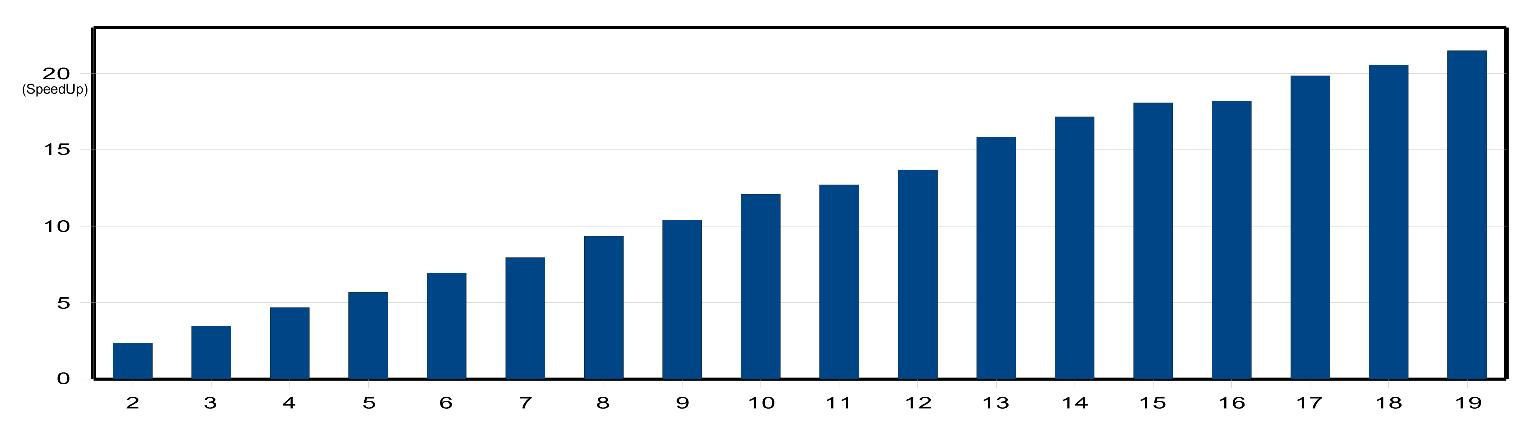
\includegraphics[width=14cm]{./../img/recogspeedup_300.eps}
\caption{Mirum est notare quam littera gothica, quam nunc putamus parum claram, anteposuerit litterarum formas humanitatis per seacula quarta decima et quinta decima \cite{OPTO-Skoczylas}.}
\label{my-scheme}
\end{figure}

Lorem ipsum dolor sit amet, consectetuer adipiscing elit, sed diam nonummy nibh euismod tincidunt ut laoreet dolore magna aliquam erat volutpat (patrz rys.~\ref{my-scheme}). 

\par
Lorem ipsum dolor sit amet, consectetuer adipiscing elit, sed diam nonummy nibh euismod tincidunt ut laoreet dolore magna aliquam erat volutpat. Ut wisi enim ad minim veniam, quis nostrud exerci tation ullamcorper suscipit lobortis nisl ut aliquip ex ea commodo consequat. Duis autem vel eum iriure dolor in hendrerit in vulputate velit esse molestie consequat, vel illum dolore eu feugiat nulla facilisis at vero eros et accumsan et iusto odio dignissim qui blandit praesent luptatum zzril delenit augue duis dolore te feugait nulla facilisi. Nam liber tempor cum soluta nobis eleifend option congue nihil imperdiet doming id quod mazim placerat facer possim assum. 

%\clearpage

\subsection{Cele pracy}
\begin{itemize}
\item Lorem ipsum dolor sit amet, consectetuer adipiscing elit, sed diam nonummy nibh euismod tincidunt ut laoreet dolore magna aliquam erat volutpat. 
\item Ut wisi enim ad minim veniam, quis nostrud exerci tation ullamcorper suscipit lobortis nisl ut aliquip ex ea commodo consequat. 
\item Duis autem vel eum iriure dolor in hendrerit in vulputate velit esse molestie consequat
\end{itemize}

\clearpage
\subsection{Plan pracy}

W rozdziale \ref{rozdzial1} oraz~\ref{podrozdzial-Lorem2} opisano Lorem ipsum dolor sit amet. W rozdziale \ref{metoda_rozdzialu2} oraz~\ref{podrozdzial-Sed} opisano Sed ut perspiciatis.


\section{Tytuł rozdziału pierwszego}
\label{rozdzial1}

\subsection{Sed ut perspiciatis}
Sed ut perspiciatis unde omnis iste natus error sit voluptatem accusantium doloremque laudantium, totam rem aperiam, eaque ipsa quae ab illo inventore veritatis et quasi architecto beatae vitae dicta sunt explicabo. Nemo enim ipsam voluptatem quia voluptas sit aspernatur aut odit aut fugit, sed quia consequuntur magni dolores eos qui ratione voluptatem sequi nesciunt. Neque porro quisquam est\footnote{qui dolorem ipsum quia dolor sit amet}, consectetur, adipisci velit, sed quia non numquam eius modi tempora incidunt ut labore et dolore magnam aliquam quaerat voluptatem. Ut enim ad minima veniam, quis nostrum exercitationem ullam corporis suscipit laboriosam, nisi ut aliquid ex ea commodi consequatur? Quis autem vel eum iure reprehenderit qui in ea voluptate velit esse quam nihil molestiae consequatur, vel illum qui dolorem eum fugiat quo voluptas nulla pariatur?

\subsection{Lorem ipsum II}
\label{podrozdzial-Lorem2}

Lorem ipsum dolor sit amet, consectetur adipisicing elit, sed do eiusmod tempor incididunt ut labore et dolore magna aliqua. Ut enim ad minim veniam, quis nostrud exercitation ullamco laboris nisi ut aliquip ex ea commodo consequat. Duis aute irure dolor in reprehenderit in voluptate velit esse cillum dolore eu fugiat nulla pariatur. Excepteur sint occaecat cupidatat non proident, sunt in culpa qui officia deserunt mollit anim id est laborum of histogram $h$.

\begin{equation}
T_k = \frac{\displaystyle\sum_{i=0}^{T_{k-1}} i*h[i]}{\displaystyle 2 \sum_{i=0}^{T_{k-1}}h[i]} 
	+ \frac{\displaystyle\sum_{i=T_{k-1}+1}^{N} i*h[i]}{\displaystyle 2 \sum_{i=T_{k-1}+1}^{N}h[i]}
\end{equation}

Momentem zatrzymania algorytmu jest spełnienie warunku:
\begin{equation}
(T_B = T_W) \vee (T_{k-1} = T_k)
\end{equation}

\begin{figure} [htb]
\centering
\ifx\imagesversion\imagesdraft
	\includegraphics[width=12cm]{./../img/recogspeedup_300_draft.eps}
\else
	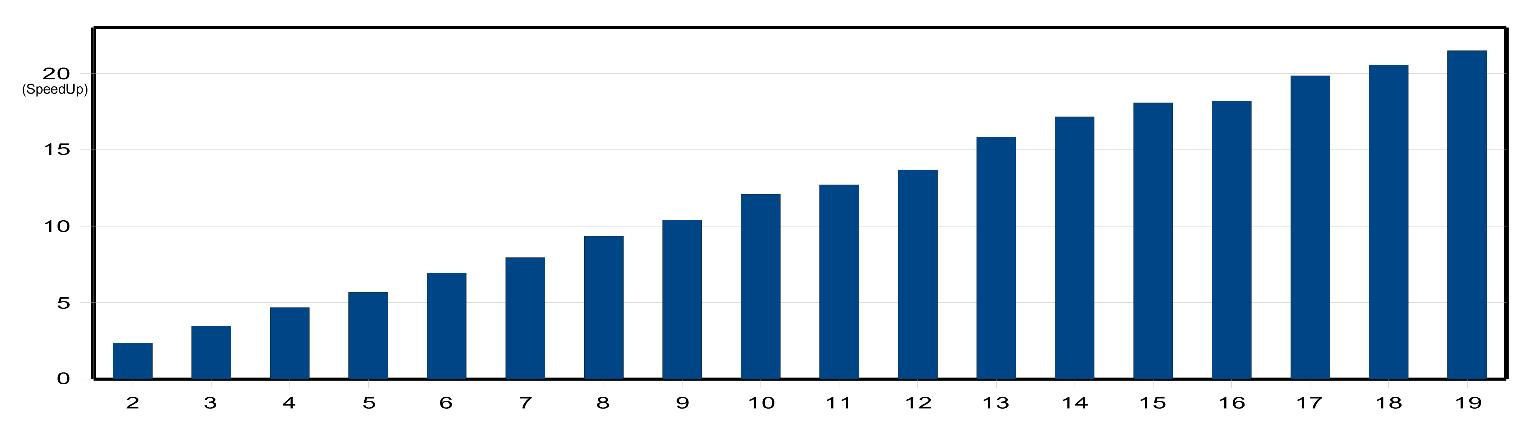
\includegraphics[width=12cm]{./../img/recogspeedup_300.eps}
\fi
\caption{Przykład przedstawia Lorem ipsum dolor sit amet (kolor niebieski)}
\label{class_selection}
\end{figure}

Przykładowe wartości statystyczne obliczone z histogramu dla wybranych obszarów: tło, brzeg komórki, wnętrze komórki przedstawione są w tabeli \ref{texture-feat-histogram}.
\begin{center}
\begin{table}[htb]	%[htb]
\label{texture-feat-histogram}
\caption{Przykładowe wartości statystyczne obliczone z histogramu dla wybranych obszarów.}
%\newcolumntype{S}{>{\centering\arraybackslash} m{.4\linewidth} }
\begin{tabular}{|c|c|c|c|c|}
\hline
\multicolumn{5}{c}{Wnętrze komórki} \\ \hline
Obraz obszaru & średnia & wariancja & skośność & kurtoza \\ \hline

\includegraphics[width=2cm]{./../img/texture-feats-examples/internal/lspot-0163-0202.eps}
	& 0.63137976 & 0.34081793 & 0.21212126 & -2.98348491 \\ \hline

\includegraphics[width=2cm]{./../img/texture-feats-examples/internal/lspot-0258-0153.eps}	
	& 0.60025141 & 0.32051886 & 0.19296321 & -2.98727716 \\ \hline
\multicolumn{5}{c}{Krawędź komórki} \\ \hline
Obraz obszaru & średnia & wariancja & skośność & kurtoza \\ \hline

\includegraphics[width=2cm]{./../img/texture-feats-examples/edge/lspot-0074-0134.eps}
	& 0.49186311 & 0.21801289 & 0.10819958 & -2.99728385 \\ \hline

\includegraphics[width=2cm]{./../img/texture-feats-examples/edge/lspot-0294-0093.eps}
	& 0.50519031 & 0.22901042 & 0.11651124 & -2.99668923 \\ \hline
\multicolumn{5}{c}{Tło} \\ \hline
Obraz obszaru & średnia & wariancja & skośność & kurtoza \\ \hline

\includegraphics[width=2cm]{./../img/texture-feats-examples/bkg/lspot-0420-0162.eps}
	& 0.49653979 & 0.21544670 & 0.10645873 & -2.99738607 \\ \hline

\includegraphics[width=2cm]{./../img/texture-feats-examples/bkg/lspot-0426-0189.eps}
	& 0.53896788 & 0.24888885 & 0.13234195 & -2.99531207 \\ \hline
\end{tabular}
\end{table}
\end{center}
%\clearpage

Proszę zwrócić uwagę na algorytm \ref{cooccurrence-algorithm}.

\begin{algorithm}
	\SetKwInOut{Input}{wejście}\SetKwInOut{Output}{wyjście}
	\Input{macierz $R$ o rozmiarze $rows\times columns$}
	\Output{macierze współwystępowania $C$}
	\BlankLine
	\For{$d\leftarrow 1$ \KwTo $distance$}
	{
		\ForEach{$\theta \in 0, \frac{2\pi}{dirs}, 2\pi$}
		{
%			\emph{zerowanie tablicy}\\
			\For{$i\leftarrow 0$ \KwTo $max~brightness$}
			{
				\For{$j\leftarrow 0$ \KwTo $max~brightness$}
				{
					$P_{d,\theta}(i, j) \leftarrow 0$\;
				}
			}
			\For{$t\leftarrow 0$ \KwTo $columns-1$}
			{
				\For{$k\leftarrow 0$ \KwTo $rows-1$}
				{
					$tc \leftarrow $floor$(t + d\cdot cos(\theta))$\;
					$kc \leftarrow $floor$(k + d\cdot sin(\theta))$\;
					\If{$(0 \leq yc)\cdot(yc < rows)\cdot(0 \leq xc)\cdot(xc < columns)$}
					{
						$C_{d,\theta}(R_{t,k},R_{tc,kc}) \leftarrow C_{d, \theta}(R_{t,k},R_{tc, kc}) + 1$\;
					}
				}
			}
		}
	}
\caption{Wyznaczanie macierzy współwystępowania}
\label{cooccurrence-algorithm}
\end{algorithm}

Po uzyskaniu macierzy współwystępowania generowane są następujące cechy:

\begin{equation}
\mu_{x} = \displaystyle\sum\limits_{m} m \displaystyle\sum\limits_{n} C_{d,\theta}(m,n)
\end{equation}

\begin{equation}
\mu_{y} = \displaystyle\sum\limits_{n} n \displaystyle\sum\limits_{m} C_{d,\theta}(m,n)
\end{equation}

\begin{equation}
\sigma_{x} = \displaystyle\sum\limits_{m}(m-\mu_x)^2 \displaystyle\sum\limits_{n} C_{d,\theta}(m,n)
\end{equation}

\begin{equation}
\sigma_{y} = \displaystyle\sum\limits_{n}(n-\mu_y)^2 \displaystyle\sum\limits_{m} C_{d,\theta}(m,n)
\end{equation}

\begin{equation}
Energy = \displaystyle\sum\limits_{m,n} C_{d,\theta}(m,n)^2
\end{equation}

\begin{equation}
Entropy = -\displaystyle\sum\limits_{m,n} C_{d,\theta}(m,n)\log(C_{d,\theta}(m,n))
\end{equation}

\begin{equation}
IDM = \displaystyle\sum\limits_{m,n}\frac{1}{1 + (m - n)^2} C_{d,\theta}(m,n)
\end{equation}

\begin{equation}
Shade = \displaystyle\sum\limits_{m,n}(m + n - \mu_x - \mu_y)^3 C_{d,\theta}(m,n)
\end{equation}

\begin{equation}
Inertia = \displaystyle\sum\limits_{m,n}(m-n)^2 C_{d,\theta}(m,n)
\end{equation}

\begin{equation}
Promenance = \displaystyle\sum\limits_{m,n}(m+n-\mu_x-\mu_y)^4 C_{d,\theta}(m,n)
\end{equation}

\begin{equation}
Correlation = -\displaystyle\sum\limits_{m,n}\frac{(m-\mu_x)(n-\mu_y)}{\sqrt{(\sigma_x \sigma_y)}} C_{d,\theta}(m,n)
\end{equation}

Do tej pory nie rozwiązywano w ten sposób problemu, zatem propozycja autora niniejszej rozprawy jest nowatorska \cite{SanFrancisco-poster}. 

%\chapter{Oj pomyliłem się to nie ten tytuł}
\chapter{Prawdziwy tytuł rozdziału 2}
\label{metoda_rozdzialu2}

\section{Sformułowanie zagadnienia}

Znane są powszechnie algorytmiczne, oparte na wiedzy eksperta, sposoby podejścia do rozwiązania problemu. Ostrość czy rodzaj lub typ --- ale takich przypadków można wymienić więcej.

\subsection{Lorem ipsum XXX}
\label{podrozdzial-Sed}

Sed ut perspiciatis unde omnis iste natus error sit voluptatem accusantium doloremque laudantium, totam rem aperiam, eaque ipsa quae ab illo inventore veritatis et quasi architecto beatae vitae dicta sunt explicabo. Nemo enim ipsam voluptatem quia voluptas sit aspernatur aut odit aut fugit, sed quia consequuntur magni dolores eos qui ratione voluptatem sequi nesciunt. Neque porro quisquam est, qui dolorem ipsum quia dolor sit amet, consectetur, adipisci velit, sed quia non numquam eius modi tempora incidunt ut labore et dolore magnam aliquam quaerat voluptatem. Ut enim ad minima veniam, quis nostrum exercitationem ullam corporis suscipit laboriosam, nisi ut aliquid ex ea commodi consequatur? Quis autem vel eum iure reprehenderit qui in ea voluptate velit esse quam nihil molestiae consequatur, vel illum qui dolorem eum fugiat quo voluptas nulla pariatur?


%\chapter*{Definicje}
\chapter{Definicje}
\begin{list}{}{\leftmargin=0em}

%\renewcommand{\labelitemi}{}
\item $\mathbb{R}$ - zbiór liczb rzeczywistych
\item $I$ - macierz opisująca obraz wejściowy
\item $w$ - szerokość obrazu wejściowego, liczba kolumn macierzy $I$
\item $h$ - wysokość obrazu wejściowego, liczba wierszy macierzy $I$
\item $I_{x,y}$ - piksel z obrazu wejściowego na pozycji x, y; wyraz macierzy w~kolumnie~$x$ i~wierszu~$y$
\item $R(x,y)$ - zbiór reprezentujący otoczenie piksela $I_{x,y}$. W przypadku gdy otoczenie ma postać kwadratu jest to macierz kwadratowa
\item $R_{t,k}(x,y)$ - element macierzy otoczenia piksela $I_{x,y}$ w kolumnie $t$ i wierszu $k$. Dla uproszczenia czasem zapisywane jako $R_{t,k}$
\item $\vec{v_{R(x,y)}}$ - wektor cech teksturalnych otoczenia $R(x,y)$
\item $\Psi$ - klasyfikator tekstur
\item $P$ - zbiór zawierający wyniki klasyfikacji otoczeń pikseli obrazu $I$. Zbiór może być reprezentowany w postaci macierzy, w której każdy element tej macierzy odpowiada wynikowi klasyfikacji otoczenia $R_{x,y}$. Rozmiar macierzy $P$ jest mniejszy niż obrazu wejściowego $I$, gdy krok przesuwania okna (kolejnych obszarów $R$) jest większy niż 1~piksel
\item $C_{d,\theta}(m,n)$ - macierz współwystępowania (ang. Co-occurrence matrix)
\item $RLM_{\theta}(i,j)$ - macierz długości ciągów (ang. Run-length matrix)

\item $S$ - zbiór zawierający zalążki segmentacji
\item $Q$ - zbiór wysegmentowanych obszarów
\item $\vec{u_{Q_i}}$ - wektor cech kształtu obszaru $Q_i$
\item $\Gamma$ - odosobniony, ciągły obszar, składający się z jednego segmentu lub wielu segmentów
\item $\Lambda$ - zbiór odosobnionych, ciągłych obszarów $\Gamma$ zdetektowanych na obrazie
\item $\vartheta$ - ciągły obszar (może, ale nie musi być odosobniony), może składać się z jednego segmentu lub wielu
\item $\Phi$ - klasyfikator obiektów (obszarów)
\item $\Theta$ - zbiór obiektów (obszarów, czyli połączonych segmentów) reprezentujący rozpoznane z~obrazu komórki. W~szczególnym przypadku obszar może składać się z~jednego segmentu.

\end{list}
\chapter*{Lista publikacji}
%\chapter{Lista publikacji}
\thispagestyle{empty}
\pagestyle{empty}

\par
\hspace{0.6cm}C. Zet, H. Kiesewetter, M. Skoczylas, L. Westerberg, R. Spohr. A system for irradiating polymer films with a preset number of ions. GSI Scientific Report, Gesellschaft f\"ur Schwerionenforschung mbH (GSI), 154, 2003

\par
C. Zet, C. Foslau, M. Skoczylas, L. Westerberg, R. Spohr. System for irradiating polymer films with a preset number of ions. SIELMEN, 4th International Conference on Electromechanical and Power Systems  vol. 2, 167-170, 2003

\par M. Skoczylas, K. Andrzejewski. Krzyżtopór. Telewizja Polska, wyd. Rzeczpospolita, Akademia Filmu i Telewizji Warszawa, 2005

\par
R. Spohr, P. Apel, H. Kiesewetter, M. Skoczylas, C. Zet. Elektrolytische Bank. Patent~DE~10~2005~020~734, 2006

\par
M. Skoczylas, R. Cherubini, S. Gerardi. Automatic unstained cells recognition for single-cell irradiations. LNL Annual Report, INFN-LNL, 61-62, 2006

\par
M. Skoczylas, R. Cherubini, S. Gerardi. Automatic unstained cells recognition for single-cell irradiations, Proceedings of the XIII International Congress of Radiation Research, San Francisco, USA, 2007

\par
M. Skoczylas, R. Cherubini, S. Gerardi. Further development of the INFN-LNL automated unstained cell recognition system for single-cell irradiations. LNL Annual Report, INFN-LNL, 2008

\par
M. Skoczylas, R. Cherubini, S. Gerardi. Automated detection system of unstained viable cells in phase-contrast microscopy. Proceedings of the 8th International Workshop on Microbeam probes of cellular radiation response, NIRS, Chiba, Japan, November 13-15, 2008, p. 5-2; Journal of Radiation Research, Vol. 50, Supplement A, A107, 2009

\par
M. Skoczylas, K. Bandurski, R. Cherubini, V. De Nadal, S. Gerardi. On-line results of the INFN-LNL automated unstained cell recognition system for single-cell irradiations. LNL Annual Report, INFN-LNL, 2009

\par
M. Skoczylas, R. Cherubini, S. Gerardi. Automatic detection of unstained viable cells in phase-contrast microscope images. Zeszyty Naukowe Politechniki Bialostockiej, zeszyt 4, 2009

\par
M. Skoczylas, W. Rakowski, R. Cherubini, S. Gerardi. Wavelet-SVM classification and automatic recognition of unstained viable cells in phase-contrast microscopy. Radiation Protection Dosimetry, Oxford Journals, 2010

\par
M. Skoczylas, W. Rakowski, R. Cherubini, S. Gerardi. Unstained viable cell recognition in phase-contrast microscopy. Opto-Electronics Review, Versita, Springer-Verlag~GmbH, 2011


\bibliography{references}
\nocite{*}
%\bibliographystyle{plain}
\bibliographystyle{unsrt}

\end{document}

